\section{Numerical examples} \label{sec:Examples}
In this section we present three numerical examples to test the method.
The first one consists of a heat equation used to illustrate the general behaviour of the reduced basis. In the second example we use the wave equation to assess the numerical properties of the method. And in the third example, we apply the method to a convection-dominated problem.

\subsection{Wave equation: Model parameters} \label{ssec:Wave}

As a first numerical example we solve the non-homogeneous wave equation
\begin{alignat}{2} \label{eq:wave}
    u_{tt} - c^2 \nabla^2 u &= b &\qquad \text{on} \; \Omega \times \setI_h \\
    u(\bm{x},t) &= u_D(\bm{x},t) = 0 &\qquad \text{on} \; \partial \Omega \times \setI_h \\
    u(\bm{x},0) &= u_0(\bm{x}) = 0 &\qquad \text{on} \; \Omega.
\end{alignat}
The domain $\Omega$ consists in a polygonal shape described by the vertices $[(0.0,0.0),(1.0,0.0),(1.0,0.3),(0.0,1.0)]$, over the time interval $\setI_h = (0,25]$. We discretize the problem using a mesh of $61204$ triangular elements and a time step $\delta t = 0.005$. As in the previous example, we define the load with its components $b_x$ and $b_t$, and the load in the frequeency domain $\widehat{b}$ as
\begin{align}
    b_x(\bm{x}) &= \exp \left(-\gamma^2 \left[(x_0-0.8)^2 + (x_1-0.15)^2 \right] \right), \\
    b_t(t) &= A \sin(\omega t) \e^{-\tau t}, \quad \widehat{b}(s) = \frac{\omega}{\omega^2 +(s+\tau)^2},
\end{align}
with $\bm{x}=[x_0,x_1]$, $\gamma=500$, $\omega=10$, $\tau=0.1$, $c=0.75$ and $A=1e4$.

The aim of this numerical example is to evaluate the behaviour of the solution for different values of $\beta$, and different sizes of the sampling set $n_s$ and the reduced basis $n_r$. As we already explore the best alternative to construct the basis in the previous example, here we choose to follow the symplectic method $\phi_{[\Re,\Im]}^{n_s}$, fixing $\alpha=1$.
In \cref{fig:wave-basisS} we show the singular value decay for $\beta = [10, 15, 25, 50]$ and sample sizes $n_s = [50, 100, 200, 500, 1000]$.

In \cref{fig:wave-contour} we show a contour plot of the solution at different time steps, here we can see the complexity of the solution and how unpredictable is its behaviour caused by the interference of the waves in the enclosed domain.

\begin{figure}[H]
	\centering
    \begin{tblr}
    {cell{1}{3} = {r=2}{},}
	\begin{subfigure}[htb!]{0.38\textwidth}
	    \centering
	    \includegraphics[width=0.9\textwidth]{figures/wave/wave-contour1.png}
        \caption{$t=23.5$} 
    \end{subfigure} &
    \begin{subfigure}[htb!]{0.38\textwidth}
	    \centering
	    \includegraphics[width=0.9\textwidth]{figures/wave/wave-contour2.png}
        \caption{$t=24.0$}
    \end{subfigure} & \includegraphics[scale=0.15]{figures/wave/wave-contour.png} \\
    \begin{subfigure}[htb!]{0.38\textwidth}
	    \centering
	    \includegraphics[width=0.9\textwidth]{figures/wave/wave-contour3.png}
        \caption{$t=24.5$} 
    \end{subfigure} &
    \begin{subfigure}[htb!]{0.38\textwidth}
	    \centering
	    \includegraphics[width=0.9\textwidth]{figures/wave/wave-contour4.png}
        \caption{$t=25.0$}
    \end{subfigure} &
    \end{tblr}
	\caption{Contour plots of the wave problem.} 
	\label{fig:wave-contour}
\end{figure}

In \cref{fig:wave-basisS}, we show the decay of the singular values $\Sigma$ for the different values of $\beta$ and $n_s$. As expected, the decay of $\Sigma$ varies with the size of the sampling set $n_s$, as we are adding more information when we increase it. It also varies significantly when we change the parameter $\beta$. This is likely caused by the fact that when we increase $\beta$ we are sampling further and further from $0$ in the line $\imath \IR$, which means that we are including higher frequencies in the sampling set that need more basis vectors to be represented adequately.
\begin{figure}[H]
	\centering
	\begin{subfigure}[htb!]{0.49\textwidth}
	    \centering
	    \input{figures/wave/wave-basis.pgf}
        \caption{$\beta=10$.} 
        \label{fig:wave-basis-b1} 
    \end{subfigure}
    \begin{subfigure}[htb!]{0.49\textwidth}
	    \centering
	    \input{figures/wave/wave-basis2.pgf}
        \caption{$\beta=15$.} 
        \label{fig:wave-basis-b2} 
    \end{subfigure} \\
    \vspace{-0.55cm}
    \begin{subfigure}[htb!]{0.49\textwidth}
	    \centering
	    \input{figures/wave/wave-basis3.pgf}
        \caption{$\beta=25$.} 
        \label{fig:wave-basis-b3} 
    \end{subfigure}
    \begin{subfigure}[htb!]{0.49\textwidth}
	    \centering
	    \input{figures/wave/wave-basis4.pgf}
        \caption{$\beta=50$.} 
        \label{fig:wave-basis-b4} 
    \end{subfigure}
    \caption{Singular values of the wave problem for multiple sample sizes $n_s$.} 
	\label{fig:wave-basisS} 
\end{figure}

To numerically evaluate the solution we define the relative $H^1(\setI,\IV)$-error as
\begin{equation} \label{eq:H1-error}
    \norm*{u_h - u_h^{\textrm{R}}}_{H^1({\setI_h,\IV_h})} = \frac{1}{n_t} \sum_{j=1}^{n_t} \left( \norm*{u_h(t_j) - u_h^{\textrm{R}}(t_j)}_{H^1({\IV_h})} \right).
\end{equation}
In \cref{fig:wave-error} we show the relative $H^1(\setI,\IV)$-error for for the time interval $\setI_h=(0,25]$, $n_t=5000$ time steps, and different values of $\beta$. \Cref{fig:wave-error-ns} displays the error convergence for sample size $n_s$, while keeping the basis size $n_r=\frac{n_s}{2}$. \Cref{fig:wave-error-nr} shows the error convergence for the reduced basis size $n_r$, fixing the sample size to $n_s=1000$.
\begin{figure}[H]
	\centering
    \begin{subfigure}[htb!]{0.49\textwidth}
     	\centering
        \input{figures/wave/wave-error-ns.pgf}
        \caption{Error convergence for $n_s$ with $n_r=\frac{n_s}{2}$ .} 
	    \label{fig:wave-error-ns}
    \end{subfigure}
    \begin{subfigure}[htb!]{0.49\textwidth}
     	\centering
        \input{figures/wave/wave-error-nr.pgf}
        \caption{Error convergence for $n_r$ with $n_s=1000$ samples.} 
	    \label{fig:wave-error-nr}
    \end{subfigure}
    \caption{$H^1$-error of the advection-dominated problem.}
	\label{fig:wave-error}
\end{figure}

Although error decreases in all the cases we find different behavior. As we increase the value of $\beta$ we are sampling higher frequencies and consequently we need a bigger amount of samples to appropriately capture the behavior of the problem. This can be seen by comparing \cref{fig:wave-basisS,fig:wave-error}, where the the point where the singular values begins to decay matches the decrease of the error. In the other hand, when we have enough samples as in \cref{fig:wave-error-ns}, the error decay slope is similar for all the cases, still requiring a bigger basis size for a bigger $\beta$.

We compare the computational cost of the solution for $\beta=10$ and sample size $n_s=1000$. In \cref{fig:wave-time} we show the computational time of the construction of the basis, the reduced solution, and the post-process for different sizes of the basis. The finite element problem is solved in $1248$ seconds, the sampling is perform in $212$ and the construction of the basis in $144$. In this case we solve frequency problem in a parallel way using 24 cores.
\begin{figure}[H]
	\centering
    \input{figures/wave/wave-time.pgf}
    \caption{Computational cost for the wave problem.}
	\label{fig:wave-time}
\end{figure}

\subsection{Heat equation: Topology} \label{ssec:Heat}

As the second numerical example we solve a heat equation in a 2D circular domain over a time interval of $\setI=(0,200]$. The domain $\Omega$ consist in three successive rings, with seven circular inclusions in the inner and outer rings. The inclusions are distributed evenly in each ring shifted by $\pi$ with respect to each other. \Cref{fig:dif-problem} shows a schematic representation of the geometry and the physical properties of the problem. \Cref{tab:dif-data} shows the geometrical and physical parameters of the problem. We discretize the problem using a mesh of $1$ triangular elements and a time step $\delta t = 0.1$.

\begin{figure}[H]
    \centering
	\begin{subfigure}[htb!]{0.49\textwidth}
	    \centering
	    \tikzset{every picture/.style={line width=0.75pt}} %set default line width to 0.75pt        

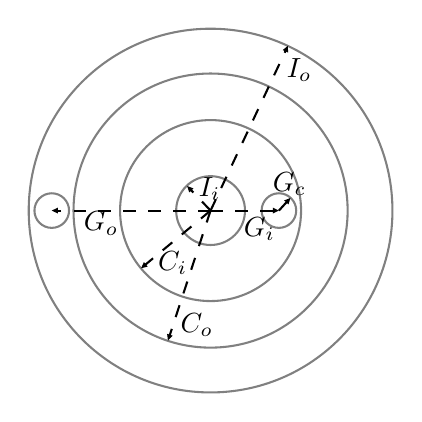
\begin{tikzpicture}[x=0.75pt,y=0.75pt,yscale=-0.55,xscale=0.55]
%uncomment if require: \path (0,493); %set diagram left start at 0, and has height of 493

%Shape: Circle [id:dp5200554260199975] 
\draw  [color={rgb, 255:red, 128; green, 128; blue, 128 }  ,draw opacity=1 ] (306.9,268.26) .. controls (306.9,180.27) and (378.22,108.95) .. (466.21,108.95) .. controls (554.19,108.95) and (625.52,180.27) .. (625.52,268.26) .. controls (625.52,356.24) and (554.19,427.57) .. (466.21,427.57) .. controls (378.22,427.57) and (306.9,356.24) .. (306.9,268.26) -- cycle ;
%Shape: Circle [id:dp9289600441081329] 
\draw  [color={rgb, 255:red, 128; green, 128; blue, 128 }  ,draw opacity=1 ] (346.15,268.26) .. controls (346.15,201.95) and (399.9,148.2) .. (466.21,148.2) .. controls (532.51,148.2) and (586.26,201.95) .. (586.26,268.26) .. controls (586.26,334.56) and (532.51,388.31) .. (466.21,388.31) .. controls (399.9,388.31) and (346.15,334.56) .. (346.15,268.26) -- cycle ;
%Shape: Circle [id:dp2722852853058765] 
\draw  [color={rgb, 255:red, 128; green, 128; blue, 128 }  ,draw opacity=1 ] (386.94,268.26) .. controls (386.94,224.48) and (422.43,188.99) .. (466.21,188.99) .. controls (509.99,188.99) and (545.48,224.48) .. (545.48,268.26) .. controls (545.48,312.04) and (509.99,347.53) .. (466.21,347.53) .. controls (422.43,347.53) and (386.94,312.04) .. (386.94,268.26) -- cycle ;
%Shape: Circle [id:dp12695243910038978] 
\draw  [color={rgb, 255:red, 128; green, 128; blue, 128 }  ,draw opacity=1 ][line width=0.75]  (436.06,268.26) .. controls (436.06,251.61) and (449.56,238.11) .. (466.21,238.11) .. controls (482.86,238.11) and (496.36,251.61) .. (496.36,268.26) .. controls (496.36,284.91) and (482.86,298.41) .. (466.21,298.41) .. controls (449.56,298.41) and (436.06,284.91) .. (436.06,268.26) -- cycle ;
%Straight Lines [id:da3446519683659942] 
\draw  [dash pattern={on 4.5pt off 4.5pt}]  (466.21,268.26) -- (447.74,248.92) ;
\draw [shift={(445.67,246.75)}, rotate = 46.32] [fill={rgb, 255:red, 0; green, 0; blue, 0 }  ][line width=0.08]  [draw opacity=0] (5.36,-2.57) -- (0,0) -- (5.36,2.57) -- cycle    ;
%Straight Lines [id:da5401882715078415] 
\draw  [dash pattern={on 4.5pt off 4.5pt}]  (466.21,268.26) -- (407.64,316.86) ;
\draw [shift={(405.33,318.78)}, rotate = 320.31] [fill={rgb, 255:red, 0; green, 0; blue, 0 }  ][line width=0.08]  [draw opacity=0] (5.36,-2.57) -- (0,0) -- (5.36,2.57) -- cycle    ;
%Straight Lines [id:da9441681184407524] 
\draw  [dash pattern={on 4.5pt off 4.5pt}]  (466.21,268.26) -- (429.82,379.26) ;
\draw [shift={(428.89,382.11)}, rotate = 288.15] [fill={rgb, 255:red, 0; green, 0; blue, 0 }  ][line width=0.08]  [draw opacity=0] (5.36,-2.57) -- (0,0) -- (5.36,2.57) -- cycle    ;
%Straight Lines [id:da066763485508196] 
\draw  [dash pattern={on 4.5pt off 4.5pt}]  (466.21,268.26) -- (532.72,126.6) ;
\draw [shift={(534,123.89)}, rotate = 115.15] [fill={rgb, 255:red, 0; green, 0; blue, 0 }  ][line width=0.08]  [draw opacity=0] (5.36,-2.57) -- (0,0) -- (5.36,2.57) -- cycle    ;
%Shape: Circle [id:dp8868545883449647] 
\draw  [color={rgb, 255:red, 128; green, 128; blue, 128 }  ,draw opacity=1 ] (510.92,268.26) .. controls (510.92,259.89) and (517.7,253.1) .. (526.07,253.1) .. controls (534.44,253.1) and (541.23,259.89) .. (541.23,268.26) .. controls (541.23,276.63) and (534.44,283.41) .. (526.07,283.41) .. controls (517.7,283.41) and (510.92,276.63) .. (510.92,268.26) -- cycle ;
%Straight Lines [id:da617491037872858] 
\draw  [dash pattern={on 4.5pt off 4.5pt}]  (466.21,268.26) -- (523.07,268.26) ;
\draw [shift={(526.07,268.26)}, rotate = 180] [fill={rgb, 255:red, 0; green, 0; blue, 0 }  ][line width=0.08]  [draw opacity=0] (5.36,-2.57) -- (0,0) -- (5.36,2.57) -- cycle    ;
%Shape: Circle [id:dp2762076315682177] 
\draw  [color={rgb, 255:red, 128; green, 128; blue, 128 }  ,draw opacity=1 ] (311.92,268.26) .. controls (311.92,259.89) and (318.7,253.1) .. (327.07,253.1) .. controls (335.44,253.1) and (342.23,259.89) .. (342.23,268.26) .. controls (342.23,276.63) and (335.44,283.41) .. (327.07,283.41) .. controls (318.7,283.41) and (311.92,276.63) .. (311.92,268.26) -- cycle ;
%Straight Lines [id:da9083670373227554] 
\draw  [dash pattern={on 4.5pt off 4.5pt}]  (466.21,268.26) -- (330.07,268.26) ;
\draw [shift={(327.07,268.26)}, rotate = 360] [fill={rgb, 255:red, 0; green, 0; blue, 0 }  ][line width=0.08]  [draw opacity=0] (5.36,-2.57) -- (0,0) -- (5.36,2.57) -- cycle    ;
%Straight Lines [id:da1774109689916481] 
\draw  [dash pattern={on 4.5pt off 4.5pt}]  (526.07,268.26) -- (534.15,259.39) ;
\draw [shift={(536.17,257.17)}, rotate = 132.3] [fill={rgb, 255:red, 0; green, 0; blue, 0 }  ][line width=0.08]  [draw opacity=0] (5.36,-2.57) -- (0,0) -- (5.36,2.57) -- cycle    ;


% Text Node
\draw (518.01,232.46) node [anchor=north west][inner sep=0.75pt]    {$G_{c}$};
% Text Node
\draw (530.41,132.46) node [anchor=north west][inner sep=0.75pt]    {$I_{o}$};
% Text Node
\draw (437.34,355.39) node [anchor=north west][inner sep=0.75pt]    {$C_{o}$};
% Text Node
\draw (417.61,301.39) node [anchor=north west][inner sep=0.75pt]    {$C_{i}$};
% Text Node
\draw (453.34,236.33) node [anchor=north west][inner sep=0.75pt]    {$I_{i}$};
% Text Node
\draw (492.67,271.79) node [anchor=north west][inner sep=0.75pt]    {$G_{i}$};
% Text Node
\draw (352.6,266.8) node [anchor=north west][inner sep=0.75pt]    {$G_{o}$};


\end{tikzpicture}

	    \caption{Geometrical parameters.}
        \label{fig:dif-problem-1}
    \end{subfigure}
    \begin{subfigure}[htb!]{0.49\textwidth}
	    \centering
	    \includegraphics[width=0.65\textwidth]{figures/dif/problem.png}
	    \caption{Physical parameters ($\mu$).}
        \label{fig:dif-problem-2}
    \end{subfigure}
    \caption{Schematic representation of the diffusion problem.}
    \label{fig:dif-problem}
\end{figure}

\begin{table}[!htb]
\centering
\caption{Geometrical and physical parameters of the diffusion problem.}
\begin{subtable}[h]{0.4\textwidth}
    \centering
    {\small
    \begin{tabular}{ccccccc}
        \toprule
        $r_w$ & $r_g^e$ & $r_g^i$ & $r_i^e$ & $r_i^i$ & $r_c^e$ & $r_c^i$  \\ \midrule  
        0.35 & 3.5 & 1.5 & 4.0 & 0.75 & 3.0 & 2.0 \\ \bottomrule
    \end{tabular}}
    \label{tab:dif-geometry}
\end{subtable}
\begin{subtable}[h]{0.3\textwidth}
    \centering
    {\small
    \begin{tabular}{ccc}
        \toprule
        $\mu_1$ & $\mu_2$ & $\mu_3$  \\ \midrule  
        0.075 & 0.5 & 27.2 \\ \bottomrule
    \end{tabular}}
    \label{tab:dif-material}
\end{subtable}
\label{tab:dif-data}
\end{table}

\pagebreak
The problem consists in solving
\begin{alignat}{2}
    \frac{\partial{u}}{\partial{t}} - \mu \Delta u &= b &\qquad \text{on} \; \Omega \times \setI \\
    u(\bm{x},t) &= 0 &\qquad \text{on} \; \Gamma \times \setI \\
    u(\bm{x},0) &= 0 &\qquad \text{on} \; \Omega. \label{eq:ht1}
\end{alignat}
We define the load using as an affine decomposition of its space and time components $b = b_x(\bm{x}) b_t(t)$. In space, we set the load as a Gaussian function located in the middle ring of the domain, and in time the load we define it as a sequence of point loads with different amplitudes. In \cref{eq:heat-load} we define the load $b$, which we illustrate in \cref{fig:dif-load}.
\begin{align}
    b_x(\bm{x}) &= \cosh \left( 25 \sqrt{2 \pi} \norm{\bm{x}} \right) \exp \left( - \frac{25 \norm{\bm{x}}^2 + 10 \pi}{2} \right)\\
    b_t(t) &= \frac{A}{\sqrt{2\cdot 10^{-4}\pi}} \exp \left( {\frac{-(t-t_0)^2}{2\cdot 10^{-4}}} \right), \label{eq:heat-load}
\end{align}
with $A = 1\cdot10^4 \cdot [1,\nicefrac{1}{2},\nicefrac{1}{4},\nicefrac{1}{8},\nicefrac{1}{16},\nicefrac{1}{32}]$, and $ t_0 = 10\cdot[0,1,2,3,4,5]$. We approximate $\mathcal{L} \{b_t\}$ as the Laplace transform of a delayed impulse $\widehat{b}(s) = \e^{-t_0s}$.

\hspace{-2mm}
\begin{figure}[H]
	\centering
	\begin{subfigure}[htb!]{0.55\textwidth}
        \centering
        \input{figures/dif/dif_load.pgf}
        \caption{$b_t$} 
        \label{fig:dif-load1}
    \end{subfigure}
    \begin{subfigure}[htb!]{0.4\textwidth}
        \centering
        \input{figures/dif/ring.pgf}
        \caption{$b_x$} 
	   \label{fig:dif-load2}
    \end{subfigure}
	\caption{Load $b$ for the diffusion problem.} 
    \label{fig:dif-load}
\end{figure}

The goal of this example is to compare the different possibilities of constructing the basis. We fix the sample size as $n_s = 250$ and the basis size $r=35$. We also set $\alpha=1$ and $\beta=10$. We define five different approaches to construct the reduced basis
\begin{itemize}
    \item Using $n_s$ real-valued samples $\bm{\mathsf{S}} = [\Re \{\widehat{u}_1 \}, \ldots, \Re \{\widehat{u}_{n_s} \}]$. We denote this basis as $\phi_\IR^{n_s}$.
    \item Using $2n_s$ real-valued samples $\bm{\mathsf{S}} = [\Re \{\widehat{u}_1 \}, \ldots, \Re \{\widehat{u}_{4n_s} \}]$. We denote this basis as $\phi_\IR^{4n_s}$.
    \item Using $n_s$ complex-valued samples $\widehat{\bm{\mathsf{S}}} = [\widehat{u}_1, \ldots, \widehat{u}_{n_s}]$, and using the real part of the obtained complex basis $\Re \{ \Phi \}$. We denote this basis as $\phi_{\Re\IC}^{n_s}$.
    \item Using $n_s$ complex-valued samples $\widehat{\bm{\mathsf{S}}} = [\widehat{u}_1, \ldots, \widehat{u}_{n_s}]$, and using the complex-valued basis $\Phi$. Note that when using this basis \cref{pr:dpr} is complex-valued. We denote this basis as $\phi_\IC^{n_s}$.
    \item Using $n_s$ complex-valued samples arranged in a real-valued set composed by the real part and imaginary part of the frequency solution as $\bm{\mathsf{S}}^S = [\Re \{\widehat{u}_1 \}, \ldots, \Re \{\widehat{u}_{n_s}\}, \Im \{\widehat{u}_1 \}, \ldots, \Im \{\widehat{u}_{n_s}\}]$. We denote this basis as $\phi_{S}^{n_s}$.
\end{itemize}

Qualitatively, all the solutions show a similar behavior with all of them approximating adequately the solution. In \cref{fig:dif-contour} we show a contour plot of the solution at $t=25$. In \cref{fig:dif-basisS} we show the singular values for all the basis. We note that the decay is exactly the same for $\phi_{S}^{n_s}$ and $\phi_\IC^{n_s}$, making a case for our claim in \cref{ssec:complexified-basis}: we can construct a real-valued reduced basis that matches the complex basis.
\begin{figure}[H]
\RawFloats
\begin{minipage}[t]{.57\textwidth}
	Under limited budget constraints, it is impractical to save all task vectors for a large number of tasks $T$. Although one could argue to only save one final merged model, we lose flexibility of task vector composition, especially when we want to only merge or unlearn a part of the knowledge from a certain task in the future. Besides, the addition performance drop as the number of tasks grows is reported in \citet{ilharco2022editing} in practice. Therefore, we propose using \textbf{task vector bases} to reduce the number of task vectors to save while retaining task information maximally and preserving the flexibility of model composition.

\begin{definition}[Task Vector Bases]
    Given $T$ task vectors, task vector bases are a new set of $d$-dimensional vectors $\{\tau_{B_1}, \dots, \tau_{B_m}\}$, where $1 < m < T$, created by applying certain transformations to the original $T$ task vectors.
    \label{def:basis}
\end{definition}

\subsection{Bases Creation}
\label{sec:bases_creation}

From \Cref{thm:task-addition}, we want $\epsilon$ to be small, thereby creating near-orthogonal bases. As observed in the green box of \Cref{fig:twice-task-orthogonality}, non-related tasks are nearly orthogonal, while similar task vectors represent certain interpretable skills. Based on this intuition, we define the transformation in \Cref{def:basis} by grouping similar task vectors using clustering algorithms to remove redundant information across tasks.

\begin{algorithm}[tb]
   \caption{Task Vector Bases Creation}
   \label{alg:task_vector_basis}
\begin{algorithmic}[1]

   \STATE {\bfseries Input:} task vectors $\tau_1, \dots, \tau_T$, inner merge methods $\texttt{merge}_\text{in}()$, threshold $\delta_1 < 0$
   \STATE $M \in \mathbb{R}^{T\times T}, M_{ij} = \cos(\tau_i,\tau_j)$ // \textit{Task clustering}
   \STATE $k = \arg\max_{1 < i \leq {T-1}} \{\lambda^{(i+1)}_{L_{|M|}} - \lambda^{(i)}_{L_{|M|}}\}$ 
   \STATE $\mathcal{C}_1, \dots, \mathcal{C}_k = $ \texttt{spectral\_cluster}$(|M|, k)$
\STATE{$\mathcal{C} = \{\}$ // \textit{Separate positive and negative directions}}
\STATE{\textbf{for} $i \in [k]$ \textbf{do}}
   \STATE \quad Extract submatrix $M_{\mathcal{C}_i}$ from $M$
   \STATE{ \quad \textbf{if} $\min{M_{\mathcal{C}_i}} < \delta_1$ \textbf{then}}
      \STATE \quad \quad $M_{\mathcal{C}_i} \mathrel{+}= |\min{M_{\mathcal{C}_i}}|$ 
      \STATE \quad \quad $\mathcal{C}_{pos}^i, \mathcal{C}_{neg}^i = $ \texttt{spectral\_cluster}$(M_{\mathcal{C}_i}, 2)$
      \STATE {\quad \quad $\mathcal{C} = \mathcal{C} \cup \{\mathcal{C}_{pos}^i, \mathcal{C}_{neg}^i\}$}
   \STATE{\quad \textbf{else} $\mathcal{C} = \mathcal{C} \cup \{\mathcal{C}_i\}$}
   \STATE $\mathcal{C}_{B_1}, \dots, \mathcal{C}_{B_m} = \mathcal{C}$  
   \STATE{\textbf{for}  $i \in [m]$ \textbf{do}}
   \STATE \quad $\tau_i = \texttt{merge}_\text{in}(\theta_0, \mathcal{C}_{B_i})$ // \textit{Create basis by merging}
   \STATE {\bfseries Return:} $\{\tau_1, \dots, \tau_{B_m}\}$
\end{algorithmic}
\end{algorithm}

\begin{table}[tb]
\caption{Bases Arithmetic. Here $i$ is a task id. There are several ways to interpret similarity search given bases and the target task.}
\label{tab:basis_arithmetic}
\centering
\scalebox{0.85}{
\begin{tabular}{@{}ll@{}}
\toprule
Arithmetic            & Expression \\ \midrule
Addition for multitask             &  $\theta^* = \texttt{merge}_\text{out}(\theta_0, \{\tau_1, \dots, \tau_{B_m}\})$.         \\
Negation for unlearning $i$       &    Find $B_j$ the most similar to $i$,    \\
       &    $\theta^* = \theta_0 - \alpha\tau_{B_j}$.       \\
OOD Generalization on $i$ &     Find $U = \{B_{j_1},\dots, B_{j_l}\}$ similar to $i$,   \\ 
 &    $\theta^* = \texttt{merge}_\text{out}(\theta_0, \{\tau_{B_{j_1}}, \dots, \tau_{B_{j_l}}\})$     \\
&    if $U = \emptyset$, store $\tau_i$ as new basis.    \\\bottomrule
\end{tabular}
}
\end{table}


In \Cref{alg:task_vector_basis}, we first create the similarity matrix of task vectors and pass this matrix into spectral clustering \citep{ng2001spectral} to group the tasks. Next, we can apply any existing merging method as $\texttt{merge}_\texttt{in}$ to create task vector bases. When cosine similarity becomes strongly negative, we first use the absolute value of the similarity for clustering and further partition the positive and negative groups with an additional clustering step. However, the scenario where task vectors have nearly opposite directions rarely occurs in practice for natural tasks unless specific adversarial tasks are defined. Therefore, lines 5-9 are typically optional. We choose spectral clustering for memory efficiency. Unlike $k$-means \citep{lloyd1982least}, which requires storing the entire set of $O(Td)$ task vectors during the update, spectral clustering only requires storing an $O(T^2)$ matrix for eigenvalue computation, which is more advantageous since $d \gg T$. Additionally, in line 3 of \Cref{alg:task_vector_basis}, we can determine the number of bases by inspecting the eigenspectrum of the Laplacian matrix $L_{|M|}$, without the need for additional hyperparameter tuning. This approach reduces the $T$ task vector addition problem to saving only $m$ task vector bases, significantly reducing the memory footprint.




\subsection{Bases Arithmetic}
\label{sec:bases_arithmetic}
 
We show how to do arithmetic with task vector bases in \Cref{tab:basis_arithmetic}, with only slight modifications from standard task arithmetic operations discussed in \Cref{sec:bounds}. There are two points that need special attention. First, we observe the usage of $\texttt{merge}_\text{out}$, which is another iteration of model merging. We can replace $\texttt{merge}_\text{out}$ easily with dataless methods such as Model Soup \cite{pmlr-v162-wortsman22a} or TIES \cite{yadav2024ties}, while for more advanced methods, we provide an example in \Cref{sec:localize-and-stitch} to show possible modifications that fit in our framework. Second, there are multiple ways to do the similarity search in \Cref{tab:basis_arithmetic}. The naive method is to fine tune $\theta_i$ till convergence to get $\tau_i$ and simply compute the cosine similarity between $\tau_i$ and bases vectors, but then one could argue to directly use $\tau_i$ for unlearning and OOD generalization. Fortunately, in \Cref{sec:intermediate}, we see without training $i$ till convergence, intermediate checkpoints even with one step of gradient update still reflects important task information. Also, as we will see in \Cref{sec:memory_70} since bases can be interpreted as some skill: for example, one bases represents digit classification and the target task is MNIST, we can use such heuristics of task similarity knowledge without any explicit computation of $\tau_i$. In these two scenarios, since $\tau_i$ is either far from the optimal or does not exist, it can be more beneficial to use stored knowledge in the bases.


	\caption{Singular values of the diffusion problem.} 
	\label{fig:dif-basisS}
\end{minipage}\hfill%
\begin{minipage}[t]{.4\textwidth}
    \includegraphics[width=\textwidth]{figures/dif/contour.png}
 	\caption{Contour plot of the diffusion problem.} 
	\label{fig:dif-contour}
\end{minipage}
\end{figure}

To compare in a more precise way the results we define the  relative $H^1(\IV)$-error as
\begin{equation} \label{eq:H1-error}
    \textrm{error}_{H^1({\IV_h})}(u_h^{\textrm{R}}) = \frac{\norm*{\nabla u_h - \nabla u_h^{\textrm{R}}}_{H^1({\IV_h})}}{\norm*{\nabla u_h}_{H^1({\IV_h})}}.
\end{equation}
In \cref{fig:dif-error} we show the evolution of the $H^1$-error for reduced solutions using the five different reduced bases. Interestingly, solving the complex-valued problem with $\phi_\IC^{n_s}$, yields the same result as using the real bases $\phi_{\Re\IC}^{n_s}$ and $\phi_{S}^{n_s}$, with $\phi_\IR^{n_s}$ having the worst approximation. We argue that this behaviour is explained by the equivalence hinted in \cref{ssec:complexified-basis}, between the reduced $\mathcal{J}$-adapted basis of $\IV_h^\IC$ and the symplectic reduced basis. Likewise, the behaviour of the real-valued basis $\phi_{\IR}^{2n_s}$ can be explained as a consequence of it being built over a sample set of the same size as for the symplectic and complex basis, but with sub-optimal sample points.
\begin{figure}[H]
	\centering
    \begin{subfigure}[htb!]{0.49\textwidth}
     	\centering
        \input{figures/dif/dif-error.pgf}
    \end{subfigure}
    \begin{subfigure}[htb!]{0.49\textwidth}
        \centering
        \input{figures/dif/dif-error2.pgf}
    \end{subfigure}
    \caption{$H^1$-error of the diffusion problem.}
	\label{fig:dif-error}
\end{figure}

In \cref{tab:dif-time} we show the computational time for the offline and online parts of the solution including the computation of the reduced basis. The computational cost of the time-dependent finite element solution is $730.8104$ and the cost of recovering the full solution from the reduced one ($\Phi \bm{\mathsf{u}}_j^{\textrm{R}}$) for all the time steps is $58.19$.
\begin{table}[!htb]
    \centering
    \caption{Computational cost of the diffusion problem solutions.}
    {\small
    \begin{tabular}{cccccc}
        \toprule
        & $\phi_{\IR}^{n_s}$ & $\phi_{\IR}^{4n_s}$ & $\phi_{\Re\IC}^{n_s}$ & $\phi_{\IC}^{n_s}$ & $\phi_{S}^{n_s}$ \\ \midrule  
        Freq & 254.9132 & 939.8105 & 254.9132 & 254.9132 & 254.9132 \\
        Basis & 26.6827 & 84.8049 & 129.7753 & 129.7753 & 44.8887 \\
        ROM & 0.4870 & 0.5020 & 0.7815 & 0.5639 & 0.4946 \\
        \bottomrule
    \end{tabular}}
\label{tab:dif-time}
\end{table}

Since we want to obtain the best approximation possible with the method while maintaining low cost, it is clear that using the symplectic construction of the reduced basis ($\phi_{S}^{n_s}$) gives the best results.
The better performance (in computational time) of this approach is due to reducing the amount of computations done as a complex-valued problem, which noticeable increase the computational cost of the other approaches.
Note that the real computational time of the frequency-domain problem can be greatly reduced as the solutions are fully independent and can be solve in parallel.



\subsection{Advection-dominated problem} \label{ssec:CDR}

In the last example we showcase some stabilization properties of the method. We solve the advection-diffusion-reaction problem
\begin{alignat}{2} \label{eq:advection}
    \frac{\partial{u}}{\partial{t}} + a \cdot \nabla u - \mu \Delta u + \kappa u &= b &\qquad \text{on} \; \Omega \times (0,t_{\textnormal{f}}] \\
    u(\bm{x},t) &= 0 &\qquad \text{on} \; \Gamma_D \times (0,t_{\textnormal{f}}] \\
    u(\bm{x},0) &= u_0(\bm{x};\mu) &\qquad \text{on} \; \Omega
\end{alignat}
with the $\mu=0.001$, $\kappa=0.1$, and the advection velocity $a=1-\abs{x_1}$. The domain $\Omega$ consists in a unit square with the boundary $\Gamma_D$ set over the edges parallel to the x-axis. The load and its Laplace transform are define as
\begin{align}
    b_x(\bm{x}) &= \exp \left(-\gamma^2 \left[(x_0-0.5)^2 + (x_1-0.5)^2 \right] \right), \\
    b_t(t) &= A t\e^{-t}\sin(\omega t), \quad \widehat{b}(s) = \frac{2\omega (s+1)}{((s+1)^2+\omega^2)^2}
\end{align}
with $A=-100$, $\omega=10\pi$, and $\gamma=25$. For the frequency domain problem we set $\alpha=1$ and $\beta=10$, and we construct the basis using $120$ samples and solve the reduced problem with $n_r=30$ basis vectors. \Cref{fig:adv-load} illustrates the load $b$ and in \cref{fig:adv-basisS} we show the singular values of the reduced basis. 
\begin{figure}[H]
\RawFloats
\begin{minipage}[t]{.49\textwidth}
	\input{figures/adv/adv-load.pgf}
	\caption{Load $b_t$ for the advection-dominated problem.} 
	\label{fig:adv-load}
\end{minipage}\hfill%
\begin{minipage}[t]{.49\textwidth}
	\input{figures/adv/adv-basis.pgf}
	\caption{Singular values of the advection-dominated problem.} 
	\label{fig:adv-basisS}
\end{minipage}
\end{figure}

In \cref{fig:adv-comparison} we compare the solutions of the finite element problem and the reduced problem at $t=0.33$. Here we can see how the instabilities have taken over the finite element solution while the reduced solution remains stable and matches the `stable part' of the high fidelity solution.

Although this property of the basis needs more analysis, we infer that the added stability is caused by filtering out the higher frequencies in both the sampling method and the \gls{svd}.
\begin{figure}[H]
	\centering
	\begin{subfigure}[htb!]{0.44\textwidth}
	    \centering
	    \includegraphics[width=\textwidth]{figures/adv/adv-fe.png}
	    \caption{Finite element solution}
    \end{subfigure}
    \begin{subfigure}[htb!]{0.44\textwidth}
	    \centering
	    \includegraphics[width=\textwidth]{figures/adv/adv-rom.png}
	    \caption{ROM solution}
    \end{subfigure}
    \begin{subfigure}[htb!]{0.1\textwidth}
	    \centering
	    \includegraphics[scale=0.085]{figures/adv/adv-label.png}
    \end{subfigure}
	\caption{Comparison of solutions for the advection-dominated problem at $t=0.33$} 
	\label{fig:adv-comparison}
\end{figure}
